\documentclass[12pt, a4paper]{book}
\begin{document}
The standard model of particle physics
\begin{equation}\label{eq:sm}
    \mathcal{L}_{SM} = -\frac{1}{4}F_{\mu\nu}F^{\mu\nu} + i\overline{\psi}\slashed{D}\psi + \psi_iy_{ij}\psi_j\phi + h.c. + \abs{D_\mu\phi}^2 - V(\phi)
\end{equation}
The elegant equation that can explain phenomena in nature with great precision. It consists of three \textit{symmetry groups}. The group explaining electromagnetism $U(1)$, the group describing the weak force $SU(2)_L$ and the group describing the strong force $SU(3)_C$. 
In this chapter we will delve into each of these gruops, the spontaneous symmetry breaking phenomena that gives mass to particles, as well as how to calculate the cross section of processes.\\
\\The theory of this section is mainly based of Peskin's and Schroeder's "An Introduction to Quantum Field Theory" \cite{Peskin:1995ev} and Thomson's "Modern Particle Physics" \cite{THOMSON}.

\clearpage
\section{Quantum Electrodynamics}
In the begining there was nothing; \textit{then God said, “Let there be light,” and there was light.} This lead us to the first part of the Standard Model, Quantum Electrodynamics, or QED for short,
\begin{equation}\label{eq:QED}
    \mathcal{L}_{QED} = \overline{\psi}\left(i\slashed{D} -m\right)\psi -\frac{1}{4}B^{\mu\nu}B_{\mu\nu}
\end{equation}
using the notation $\slashed{D}\equiv \gamma^\mu D_\mu$ where $iD_\mu = i\partial_\mu -eB_\mu$ is the covariant derivative and $B_{\mu\nu}=\partial_\mu B_\nu - \partial_\nu B_\mu$ is the electromagnetic field tensor\footnote{Taking $\partial_\mu B^{\mu\nu} = 0$ gives all of Maxwells equations.}. 
$B_\mu$ is the vector potential of the Lagrangian.\\ 
\\The above Lagrangian is part of a $U(1)$ symmetry group, meaning that there is only one unique gauge freedom, this is the rotation of phase angle of the field $\theta$. The $m$ is the mass of the \textit{Dirac} particle described by the Dirac field $\psi$.

\section{Yang-Mills Theory}
While QED is expressed by the Lagrangian in Eq. \ref{eq:QED}, which is part of a $U(1)$ symmetry group, it can still be described by a more general Lagrangian using \textit{Yang-Mills} theory
\begin{equation}\label{eq:YM_lag}
    \mathcal{L}_{YM} = \overline{f}\left(i\slashed{D} -m\right)f -\frac{1}{4}(F^a_{\mu\nu})^2
\end{equation}
where we use the notation $f\equiv\begin{pmatrix}
    f_1\\f_2\\\vdots\\f_n
\end{pmatrix}$ where $f_i$ is a field. The Yang-Mills Lagrangian looks almost identical to the QED Lagrangian, the differences being that the gauge freedom changes from a rotation of the phase angle $\theta$ to a more general
$$
\psi \rightarrow \left(1+i \alpha^a t^a + \mathcal{O}(\alpha^2)\right) \psi
$$ 
This also changes the vector fields $A_\mu^a$ such that it transforms 
$$
A_\mu^a \rightarrow A^a_\mu +\frac{1}{g}\partial_\mu\alpha^a +f^{abc}A_\mu^b\alpha^c
$$
where $e$ is replaced for a more general scale factor $g$, and $f^{abc}$ is a set of numbers called the \textit{structure constants}. From these changes follow that
$$
iD_\mu = i\partial_\mu -eA_\mu\rightarrow iD_\mu = i\partial_\mu -gA^a_\mu t^a
$$
The important thing to note about the Yang-Mills is that the covariant derivative can be \textit{non Abelian}, meaning that 
$$
\left[D_\mu,D_\nu\right] = -igF_{\mu\nu}^at^a
$$
this new $t^a$ factor is a Lie algrbra generator, which for our purposes represent a local gauge symmetry we have on the field. The structure constant has to fullfull the criteria that
\begin{equation}\label{eq:struc_const}
    [t^a,t^b]=if^{abc}t^c
\end{equation}The difference between the Yang-Mills Lagrangian is most noticable when fully writing
$$
F_{\mu\nu}^a = \partial_\mu A_\nu^a -\partial_\nu A_\mu^a +gf^{abc}A_\mu^b A_\nu^c
$$
Giving that equatin of motion
\begin{equation}\label{eq:YM_eq}
    \partial^\mu F^a_{\mu\nu} +gf^{abc}A^{b\mu}F^c_{\mu\nu} = -g\overline{\psi}\gamma_\nu t^a\psi
\end{equation}
Using Noether's thoere on the Langrangian gives us the conserved quantity of the symmetry group. There is also a theorem that states that for a $SU(n)$ symmetry group there are $n^2-1$ vector fields.\\
\\If we were to choose $U(1)$ as our local symmetry group the generator $t^a = \mathbb{I}$ and all the structure constants to be $f^{abc}=0$, meaning that we get the QED back. 
Noether's theorem also states that the conserved quantity of the Lagrangian is the electric charge $e$.

\section{Weak theory}
Using the Yang-Mills Lagrangian from Eq. (\ref{eq:YM_lag}) on a $SU(2)$, choosing $t^a =\frac{\sigma^i}{2}$, where $\sigma^i$ are the Pauli matrices, and the structure constants to be the Levi-Civita $f^{abc}=\epsilon^{ijk}$. Where $i,j,k\in[1,2,3]$.
The Weak theory gives us the gauge freedoms of
$$
\psi \rightarrow \left(1+i \alpha^i \sigma^i + \mathcal{O}(\alpha^2)\right) \psi
$$ 
Using the notation of $A_\mu\rightarrow W_\mu$ we get that there are $2^2-1$, meaning three vector fields 
$$
W_\mu^i \rightarrow W^i_\mu +\frac{1}{g}\partial_\mu\alpha^i +\epsilon^{ijk}W_\mu^j\alpha^k
$$
If one were to apply Noether's theorem on this Lagrangian we would get that two quantities are conserves, the \textit{hypercharge} and \textit{isospin}.


\section{Quantum Chromodynamics}
Using the Yang-Mills Lagrangian from Eq. (\ref{eq:YM_lag}) on a $SU(3)$, choosing $t^a =\frac{\lambda^a}{2}$, where $\lambda^a$, the \textit{Gell-Mann matrices}, are the equivalent of the SU(2) Pauli matrices:
\begin{align}\label{eq:Gell-Mann}
    \begin{split}
        \lambda ^{1}={\begin{pmatrix}0&1&0\\1&0&0\\0&0&0\end{pmatrix}},\quad 
        \lambda ^{2}={\begin{pmatrix}0&-i&0\\i&0&0\\0&0&0\end{pmatrix}},\quad 
        \lambda ^{3}={\begin{pmatrix}1&0&0\\0&-1&0\\0&0&0\end{pmatrix}}, \\\\
        \lambda ^{4}={\begin{pmatrix}0&0&1\\0&0&0\\1&0&0\end{pmatrix}},\quad 
        \lambda ^{5}={\begin{pmatrix}0&0&-i\\0&0&0\\i&0&0\end{pmatrix}},\quad 
        \lambda ^{6}={\begin{pmatrix}0&0&0\\0&0&1\\0&1&0\end{pmatrix}}, \\\\
        \lambda ^{7}={\begin{pmatrix}0&0&0\\0&0&-i\\0&i&0\end{pmatrix}},\quad 
        \lambda ^{8}={\frac {1}{\sqrt {3}}}{\begin{pmatrix}1&0&0\\0&1&0\\0&0&-2\end{pmatrix}}
    \end{split}
\end{align} 
as the structure constant has to obey Eq. (\ref{eq:struc_const}) we get 
\begin{align*}
    f^{123}=1\\
    f^{147}=-f^{156}=f^{246}=f^{257}=f^{345}=-f^{367}={\frac{1}{2}}\\
    f^{458}=f^{678}={\frac {\sqrt {3}}{2}}
\end{align*}
Using the notation of $A_\mu\rightarrow G_\mu$ we get that there are $3^2-1$, meaning \textit{eight} vector fields 
$$
G_\mu^a \rightarrow G^a_\mu +\frac{1}{g}\partial_\mu\alpha^a +\epsilon^{abc}G_\mu^b\alpha^c
$$
If one were to use Noether's theorem on the $SU(3)$ Yang-Mills Lagrangian, we would get that there are thre conserved quantities for this symmetry group. These are the colors, $r,g$ and $b$. With all the information above we can 
fully describe Quantum Chrono Dynamics, which describe quark interactions. The eight vector fields are the eight different gluons that are in the theory.\\
\\In this theory we have color triplets
$$
f=\begin{pmatrix}
    f_1\\f_2\\f_3
\end{pmatrix}
$$
where $f_i$ is the color state of the particle we are studying.

\section{Electroweak unification and the BEH Mechanism}
We have so far explained the three symmetry groups that form the SM, but this is not the full picture yet. To get the full SM we need to talk about the electroweak $U(1)_Y\otimes SU(2)_L$ unification that can be explained when studying the spontaneous symmmetry breaking (SSB) phenomena, 
which also includes the \textit{Higgs} boson. \\
\\If we introduce a new complex scalar field $\phi$ that transforms in the $SU(2)$ representation, we can write the Lagrangian
\begin{equation}\label{eq:electroweak}
    \mathcal{L}=-\frac{1}{2}\Tr\left(W_{\mu\nu}W^{\mu\nu}\right)-\frac{1}{4}B_{\mu\nu}B^{\mu\nu}+\left(D_\mu \phi\right)^\dagger\left(D^\mu \phi\right) -\lambda\left(\phi^\dagger \phi -\frac{v^2}{2}\right)^2
\end{equation}
with 
\begin{equation}\label{eq:covar_higgs}
    D_\mu \phi =\partial_\mu \phi -igW_\mu^a\sigma^a-i\frac{e}{2}B_\mu \phi
\end{equation}
where $W_\mu$ and $B_\mu$ are vector fields of the $SU(2)$ and $U(1)$ group respectively. And where $ -\lambda\left(\phi^\dagger \phi -\frac{v^2}{2}\right)^2 = V(\phi)$ is the potential of the new complex scalar field. 
Writing 
\begin{equation}\label{eq:Higgs}
    \phi = \begin{pmatrix}
        o\\v+H(x)
    \end{pmatrix}
\end{equation}
where $H$ is real scalar field, expands the potential to be
\begin{equation}\label{eq:sombrero}
    V(H) =\frac{1}{2}m_H^2H^2 + \frac{1}{2v}m_H^2H^3 +\frac{1}{8v^2}m_H^2H^4
\end{equation}
where we have used that $m_H = \sqrt{2\lambda}v$. This potential is the so-called \textit{Sombrero potential} and we can reveal that this scalar field $H$ is the Higgs boson. 
The consequences of writing our complex scalar field using Eq. \ref{eq:Higgs} comes when from the shape of the potential\todo{Should I add a figure?}, this gives rise to the mass of particles. The SSB comes from the fact that the fields have two minima 
on the potential but can move around in a higher dimensional space (around the sombreo edge) to get to the other minima. To explicitly show how this SSB phenomena gives mass to particles one can do a unitary gauge transormation of the scalar field, and 
this would ass mass terms to every particle that interacts with the Higgs field on the Lagrangian.\\
\\Another thing that follows from Eq. (\ref{eq:Higgs}) is that expanding on Eq. (\ref{eq:covar_higgs}) gives rise (after a lot of math) to the following relations
\begin{equation}\label{eq:W_boson}
    W_\mu^\pm = \frac{W_\mu^1 \mp iW_\mu^2}{\sqrt{2}}
\end{equation}
\begin{equation}\label{eq:Z_boson}
    Z_\mu = \frac{gW_\mu^3 - eB_\mu}{\sqrt{g^2+e^2}}
\end{equation}
\begin{equation}\label{eq:photon}
    A_\mu = \frac{gB_\mu - eW_\mu^3}{\sqrt{g^2+e^2}}
\end{equation}
These are the $W$ and $Z$ boson as well as the photon, respectively. It also adds an extra term on the Lagrangian called the $Yukawa$ Lagrangian
$$
\mathcal{L}_{YU} = \psi_i y_{ij}\psi_j\phi = \overline{U}_L G_u U_R \phi^0 + \overline{D}_L G_u U_R \phi^- \overline{U}_L G_D D_R \phi^+ \overline{D}_L G_u D_R \phi^0
$$
where $G_{u,d}$ is the Yukawa coupling and as we are looking at a complex scalar field in the $SU(2)$ representation we have from the Yang-Mills theory that we can write
$$
f=\begin{pmatrix}
    U\\D
\end{pmatrix}
$$
where $U,D$ is the field \textit{up and down} spinor. For example this can be the quark two component spinor $Q = \begin{pmatrix}
    u\\ d
\end{pmatrix}$ consisting of the $up$ and $down$ quark. The standard for weak interactions is to define $right$ and $left$ handed helicty using the operators 
$$
L = \frac{1}{2}(\mathbb{I} - \gamma_5),\qquad\text{and}\quad R = \frac{1}{2}(\mathbb{I} + \gamma_5)
$$
where $\gamma_{5}=i\gamma^0\gamma^1\gamma^2\gamma^3$. Such that we can write 
$$
U_L = L\begin{pmatrix}
    U\\D
\end{pmatrix} = \begin{pmatrix}
    U\\0
\end{pmatrix},\qquad\text{and}\quad D_R = R\begin{pmatrix}
    U\\D
\end{pmatrix} = \begin{pmatrix}
    0\\D
\end{pmatrix}
$$
as well as their hermittian conjugates. 


\section{S-matrix expansion}
But how do we calculate processes? To explain this geenrally, we can conduct an S-matrix expansion. To be more precise and use terms from quantum field theory rather than quantum mechanics, we can use the scattering operator $\mathcal{S}$ on the ineraction 
term of the SM Lagrangian $\mathcal{L}_{int}$. Starting by defining the general operator
\begin{align}\label{eq:S-matrix}
    \begin{split}
        \mathcal{S} = \sum_{i = vertices}\mathcal{S}^{(i)},\qquad\text{where}\quad \mathcal{S}^{(0)} = \mathbb{I}\qquad\text{and}\quad \\
        \mathcal{S}^{(n)}=(-i)^n\mathcal{T}\int_{-\infty}^{\infty}d^4\mathbf{x}_1\cdots\int_{-\infty}^{\infty}d^4\mathbf{x}_n\left[\mathcal{H}_{int}(x_1)\cdots\mathcal{H}_{int}(x_n)\right]
    \end{split}
\end{align}
where $\mathcal{T}$ is the \textit{time operator} ordering the terms such that we calculate our desired process, $\mathcal{H}_{int}=-\mathcal{L}_{int}$ is the interaction Lagrangian, and $\mathbf{x}_i$ are coordinates in spacetime.  The $\mathcal{S}$ operator sums over all \textit{vertices} 
of a \textit{Feynman diagram}. To calcuate the probability amplitude we can start with an easy example using QED, the Bhabha scattering process $e^- e^+\rightarrow e^-e^+$. The interaction Lagrangian in that gives us this scattering process is 
$\mathcal{L}_{int} = e\overline{\psi}(x)\gamma^\mu\psi(x)A_\mu$. To calculate the the probability amplitude we use the scattering operator in the following way
$$
\bra{f}\mathcal{S}^{(n)}\ket{i} \rightarrow \bra{e^-e^+}S^{(2)}\ket{e^-e^+} 
$$
$$
= \bra{e^-e^+}\left(-e^2\mathcal{T}\int_{-\infty}^{\infty}d^4\mathbf{x} \int_{-\infty}^{\infty}d^4\mathbf{y} \overline{\psi}(x)\gamma^\mu\psi(x)A_\mu(x)\overline{\psi}(y)\gamma^\nu\psi(y)A_\nu(y) \right)\ket{e^-e^+}
$$
Starting by using the time operator $\mathcal{T}$ on the integrals, which gives us the \textit{normal order} of the operations, we can start by using \textit{Wicks theorem} to "connect" the two points in spacetime $\mathbf{x}$ and $\mathbf{y}$. As we know there are no photons on the intial or final state, we can connect the photons as \textit{propagators}, meaning
$$
\mathcal{S}^{(2)} = -\frac{e^2}{2}\int_{-\infty}^{\infty}d^4\mathbf{x} \int_{-\infty}^{\infty}d^4\mathbf{y} \mathcal{N} \left(\wick{\overline{\psi}(x)\gamma^\mu\c1A_\mu(x)\psi(x)\overline{\psi}(y)\gamma^\nu\c1A_\nu(y)\psi(y)}\right)
$$
where 
$$
\wick{\c1A_\mu(x)\c1A_\nu(y)} = \bra{0}\mathcal{T}(A_\mu(x)A\nu(y))\ket{0} = \cdots = D_{\mu\nu}^F(x-y) = \int_{-\infty}^{\infty}\frac{d^4q}{(2\pi)^4}D_{\mu\nu}^F(q)e^{-iq(x-y)}
$$
with
\begin{equation}\label{eq:p-prop}
    D_{\mu\nu}^F(k) = \frac{-g_{\mu\nu}+r_{\mu\nu}}{(q^2+i\epsilon)}
\end{equation}
Here we have omitted the methematical details, but to summarize it with words. We calculated the photon propagator which connects two spacetime points $\mathbf{x}$ and $\mathbf{y}$ by calculating the Greens function of the Minkwoski space using among other the residue theorem from complex analysis. 
If we were now to define $\ket{e^-e^+}, \bra{e^-e^+}, \overline{\psi}$ and $\psi$ we could directly calculate the scattering amplitude by setting in the values, as this usually involves solving integrals that use Dirac delta function\footnote{At least while omitting loops, which we will do in this thesis}. 
To complete our example we define
$$
\ket{e^-e^+} = (\sqrt{2E_p}a^\dagger_{p})(\sqrt{2E_k}b_{k})\ket{0},\qquad\text{and}\quad \bra{e^-e^+} = (2\sqrt{E_pE_k})\bra{0}a_{p}b^\dagger_{k}
$$
where $E_i$ is the energy of the particle and $a_i,b_i$ and $a^\dagger_i,b^\dagger_i$ are creation and annihilation operators, respectively. In general fermion fields have
$$
\psi \equiv\int\frac{d^3p}{(2\pi)^3}\frac{1}{\sqrt{2E_\mathbf{p}}}\left(\sum_sa^s_\mathbf{p}u^s(p)e^{-ip\cdot x}+b^{s\dagger}_\mathbf{p}v^s(p)e^{ip\cdot x}\right) =\psi^+_p+\psi^-_p
$$
where depending $\psi^+$ (for $u(p)$) and $\psi^-$ (for $v(p)$) are the particle and anti-partice fields\todo{check if that is the real name}, respectively. It is standard convention to say that ingoing particles and anti-particles 
on an interaction are written as $\psi^+$ and $\overline{\psi}^-$, respectively, and their hermittian conjugate when they are outgoing. With this information we can connect the initial and final particles to their fields, solving the bra we have
$$
\bra{e^-e^+}\overline{\psi}(x)\psi(x) = (2\sqrt{E_pE_k})\bra{0}a_{p}b^\dagger_{k}\overline{\psi}^-_{k'}\psi^+_{p'},
$$
Giving
$$
\textstyle\bra{e^-e^+}\overline{\psi}(x)\psi(x) = \bra{0} \int\frac{d^3p'}{(2\pi^3)}\int\frac{d^3k'}{(2\pi^3)}\sqrt{\frac{E_pE_k}{E_{p'}E_{k'}}} \left(\sum_{s,t}a^{\dagger,s}_\mathbf{p'}u^s(p')e^{-ip'\cdot x} + b^{t}_\mathbf{k'}\overline{v}^t(k')e^{-ik'\cdot x}\right)a_{p}b^\dagger_{k}
$$
using the relation $a_{p's}a_{pt}^\dagger = (2\pi)^2\delta^{(3)}(p'-p)- a_{p's}^\dagger a_{pt}$ where the latter part kills vacuum, we get
$$
\bra{e^-e^+}\overline{\psi}(x)\psi(x) = u(x)\overline{v}(x)\bra{0}
$$
Doing the same for the ket, and setting all of this into the intial equation we get
$$
\bra{f}\mathcal{S}^{(n)}\ket{i} = -\frac{e^2}{2}\bra{0}\int_{-\infty}^{\infty}d^4\mathbf{x} \int_{-\infty}^{\infty}d^4\mathbf{y} u(x)\gamma^\mu\overline{v}(x)D_{\mu\nu}^F(x-y)\overline{u}(y)\gamma^\nu v(y)\ket{0}
$$
Giving us
$$
(2\pi)^4\delta^{(4)}(p_1+p_2-p'_1-p'_2)\overline{v}(p_1)\gamma^\mu u(p_2) \frac{g_{\mu\nu}}{q^2}\overline{u}(p'_1)\gamma^\nu v(p'_2)
$$
we can relate the scattering amplitude to a variable called the \textit{matrix amplitude}\todo{is this the real name}, $\mathcal{M}_{fi}$ by using 
$$
\bra{f}\mathcal{S}\ket{i} = i(2\pi)^4\delta^{(4)}\left(\sum_i p_i -\sum_f p_f\right)\mathcal{M}_{fi}
$$
Meaning that we have
$$
\mathcal{M}_{bhabha} = \overline{v}(p_1)\gamma^\mu u(p_2) \frac{g_{\mu\nu}}{q^2}\overline{u}(p'_1)\gamma^\nu v(p'_2)
$$
The reason we did all this is because we can calculate the \textit{differential cross section} (in the centre of mass frame) from this, using
\begin{equation}\label{eq:diff_cross}
    \frac{d\sigma}{d\Omega} = \frac{1}{64\pi^2s}\frac{p_f*}{p_i*}\abs{\mathcal{M}_{fi}}^2
\end{equation}
where $p_f*$ and $p_i*$ are the magnitudes of the final- and initial-state momenta, respectively. From the differential cross section we can also calculate the cross section by integrating over $d\Omega$. \\
\\This method is a general way to calculate the cross section of an event we want to study, but usually one just constructs the matrix element $\mathcal{M}_{fi}$ from \textit{Feynman diagrams}. In this calculation we 
already introduced the photon propagator in Eq. (\ref{eq:p-prop}), and we implicitly simplified it to be $\frac{g_{\mu\nu}}{q^2}$, which is valid for our purposes, and can be used in any event where the photon is the propagator. 
Feynman realized this and made Feynman rules to construct diagrams. The rules are shown in Figure \ref{fig:feynman_rules}. \\
\graphicspath{{../../figures/}}
\begin{figure}[!ht]
    \centering
    \includegraphics[width=\textwidth]{feynman_rules.png}
    \caption[Standard Model Feynman Rules]{The Standard Model Feynman rules. Image taken from Thomsons "Modern Particle Physics" \cite{THOMSON}}\label{fig:feynman_rules}
\end{figure}
\\Meaning that following these rules we just constructed the Feynman diagram for Bhabha scattering shown in Figure \ref{fig:bhabha}
\begin{figure}[!ht]
    \centering
    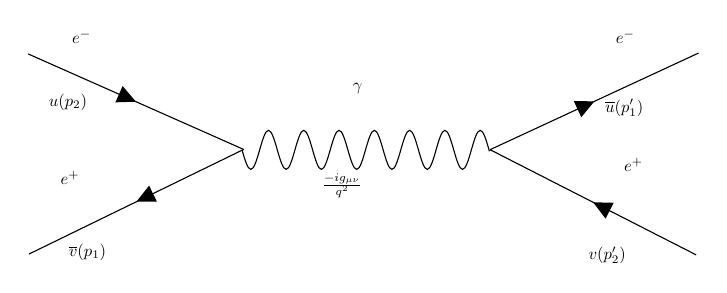
\begin{tikzpicture}[x=0.75pt,y=0.75pt,yscale=-1,xscale=1]
        %uncomment if require: \path (0,261); %set diagram left start at 0, and has height of 261
        
        %Straight Lines [id:da7156319649068418] 
        \draw    (187.8,71.6) -- (291.6,117.6) ;
        \draw [shift={(239.7,94.6)}, rotate = 203.9] [fill={rgb, 255:red, 0; green, 0; blue, 0 }  ][line width=0.08]  [draw opacity=0] (8.93,-4.29) -- (0,0) -- (8.93,4.29) -- cycle    ;
        %Straight Lines [id:da9487270827846886] 
        \draw    (291.6,117.6) -- (188.18,168) ;
        \draw [shift={(239.89,142.8)}, rotate = 334.02] [fill={rgb, 255:red, 0; green, 0; blue, 0 }  ][line width=0.08]  [draw opacity=0] (8.93,-4.29) -- (0,0) -- (8.93,4.29) -- cycle    ;
        %Shape: Wave [id:dp2508951784339145] 
        \draw   (290.8,117.8) .. controls (292.19,122.62) and (293.51,127.2) .. (295.05,127.2) .. controls (296.59,127.2) and (297.91,122.62) .. (299.3,117.8) .. controls (300.69,112.98) and (302.01,108.4) .. (303.55,108.4) .. controls (305.09,108.4) and (306.41,112.98) .. (307.8,117.8) .. controls (309.19,122.62) and (310.51,127.2) .. (312.05,127.2) .. controls (313.59,127.2) and (314.91,122.62) .. (316.3,117.8) .. controls (317.69,112.98) and (319.01,108.4) .. (320.55,108.4) .. controls (322.09,108.4) and (323.41,112.98) .. (324.8,117.8) .. controls (326.19,122.62) and (327.51,127.2) .. (329.05,127.2) .. controls (330.59,127.2) and (331.91,122.62) .. (333.3,117.8) .. controls (334.69,112.98) and (336.01,108.4) .. (337.55,108.4) .. controls (339.09,108.4) and (340.41,112.98) .. (341.8,117.8) .. controls (343.19,122.62) and (344.51,127.2) .. (346.05,127.2) .. controls (347.59,127.2) and (348.91,122.62) .. (350.3,117.8) .. controls (351.69,112.98) and (353.01,108.4) .. (354.55,108.4) .. controls (356.09,108.4) and (357.41,112.98) .. (358.8,117.8) .. controls (360.19,122.62) and (361.51,127.2) .. (363.05,127.2) .. controls (364.59,127.2) and (365.91,122.62) .. (367.3,117.8) .. controls (368.69,112.98) and (370.01,108.4) .. (371.55,108.4) .. controls (373.09,108.4) and (374.41,112.98) .. (375.8,117.8) .. controls (377.19,122.62) and (378.51,127.2) .. (380.05,127.2) .. controls (381.59,127.2) and (382.91,122.62) .. (384.3,117.8) .. controls (385.69,112.98) and (387.01,108.4) .. (388.55,108.4) .. controls (390.09,108.4) and (391.41,112.98) .. (392.8,117.8) .. controls (394.19,122.62) and (395.51,127.2) .. (397.05,127.2) .. controls (398.59,127.2) and (399.91,122.62) .. (401.3,117.8) .. controls (402.69,112.98) and (404.01,108.4) .. (405.55,108.4) .. controls (407.09,108.4) and (408.41,112.98) .. (409.8,117.8) .. controls (409.87,118.03) and (409.93,118.26) .. (410,118.49) ;
        %Straight Lines [id:da704083091568041] 
        \draw    (509.6,168.4) -- (410.31,117.72) ;
        \draw [shift={(459.96,143.06)}, rotate = 27.04] [fill={rgb, 255:red, 0; green, 0; blue, 0 }  ][line width=0.08]  [draw opacity=0] (8.93,-4.29) -- (0,0) -- (8.93,4.29) -- cycle    ;
        %Straight Lines [id:da7506662959061442] 
        \draw    (410.31,117.72) -- (510.78,71.15) ;
        \draw [shift={(460.55,94.43)}, rotate = 155.13] [fill={rgb, 255:red, 0; green, 0; blue, 0 }  ][line width=0.08]  [draw opacity=0] (8.93,-4.29) -- (0,0) -- (8.93,4.29) -- cycle    ;
        
        % Text Node
        \draw (208.2,59.2) node [anchor=north west][inner sep=0.75pt]  [xscale=0.6,yscale=0.6]  {$e^{-}$};
        % Text Node
        \draw (202.6,127.2) node [anchor=north west][inner sep=0.75pt]  [xscale=0.6,yscale=0.6]  {$e^{+}$};
        % Text Node
        \draw (343.4,84.8) node [anchor=north west][inner sep=0.75pt]  [xscale=0.6,yscale=0.6]  {$\gamma $};
        % Text Node
        \draw (474.2,121.2) node [anchor=north west][inner sep=0.75pt]  [xscale=0.6,yscale=0.6]  {$e^{+}$};
        % Text Node
        \draw (470.2,59.2) node [anchor=north west][inner sep=0.75pt]  [xscale=0.6,yscale=0.6]  {$e^{-}$};
        % Text Node
        \draw (328.6,128.4) node [anchor=north west][inner sep=0.75pt]  [xscale=0.6,yscale=0.6]  {$\frac{-ig_{\mu \nu }}{q^{2}}$};
        % Text Node
        \draw (197,90) node [anchor=north west][inner sep=0.75pt]  [xscale=0.6,yscale=0.6]  {$u( p_{2})$};
        % Text Node
        \draw (206.6,162.4) node [anchor=north west][inner sep=0.75pt]  [xscale=0.6,yscale=0.6]  {$\overline{v}( p_{1})$};
        % Text Node
        \draw (465,92.8) node [anchor=north west][inner sep=0.75pt]  [xscale=0.6,yscale=0.6]  {$\overline{u}( p'_{1})$};
        % Text Node
        \draw (457,164) node [anchor=north west][inner sep=0.75pt]  [xscale=0.6,yscale=0.6]  {$v( p'_{2})$};
        
        
    \end{tikzpicture}
    \caption{Bhabha scattering Feynman diagram}\label{fig:bhabha}
\end{figure}

\clearpage

\section{Adding it all up}
Combining the three groups $U(1)_Y\otimes SU(2)_L\otimes SU(3)_C$ as well as introducing the Higgs field from Eq. (\ref{eq:Higgs}) gives us the SM Lagrangian
$$
    \mathcal{L}_{SM} = -\frac{1}{4}F_{\mu\nu}F^{\mu\nu} + i\overline{\psi}\slashed{D}\psi + \psi_iy_{ij}\psi_j\phi + h.c. + \abs{D_\mu\phi}^2 - V(\phi)
$$
All of this is great at explaining what we know so far, which is depicted in Figure \ref{fig:SM}
\begin{figure}[!ht]
    \centering
    \includegraphics[width=0.75\textwidth]{SM.jpeg}
    \caption[The Standard Model]{The Standard Model of particle physics. Image taken from Wikipedia \textbf{[how to cite]}}\label{fig:SM}
\end{figure}
\\From Figure \ref{fig:SM} we can see all the particles on the standard model. These include the quarks $u,d,c,s,t$ and $b$, the leptons $e,\mu$ and $\tau$ as well as their neutrino partner\footnote{Since neutrinos only interact via the weak force it is only present in a field doublet}, the carrier of the strong force $g$, the carriers of the weak force $W^\pm$ and $Z$, 
the carrier of the electromagnetic force $\gamma$ and the Higgs boson $H$. From the figure we can also see which particles can interact with each of the bosons. \\
\\These are the building blocks of nature, as mesons, subatomic particles consisting of two quarks, and baryons, meaning subatomic particles consisting of three quarks (such as the proton and neutron) can furhter build atoms with eletrons to furthermore create chemistry via 
quantum mechanical processes. 


\end{document}